\documentclass[10pt,letterpaper]{article}
\usepackage[utf8]{inputenc}
\usepackage[T1]{fontenc}
\usepackage[english]{babel}
\usepackage{graphicx}
\usepackage{tocloft}
\renewcommand{\cftpartleader}{\cftdotfill{\cftdotsep}}
\renewcommand{\cftsecleader}{\cftdotfill{\cftdotsep}}
\usepackage[usenames, dvipsnames]{color}
\usepackage[framemethod=tikz]{mdframed}
\usepackage{geometry}
\geometry{hmargin=2.5cm,vmargin=2.5cm}
\title{\vspace{\fill}Microchip-CSS-Optimizer Documentation}
\author{Thibaut Meric}
\date{12.02.2015\vspace{\fill}}

\begin{document}
\maketitle
\newpage

\part {Introduction}
\setcounter{section}{0}
\section {Requirements}

This documentation is meant to help the users of Microchip-CSS-Optimizer to set up and start using the software easily.

This program was written in Python, and is compatible with Python 2.xx and Python 3.xx.It was tested under Windows 10 and Mac Os X 10.11.1 El Capitan. In order to run this program, Python must be installed on your computer.The installer is a .whl file. To run the installer, Pip must be installed on your computer.

\section {Foreword}

To build Web-pages, the Web-browser  needs a file called an HTML file. This file will gather all the text that need to be displayed to the user. In order to make the display more user friendly, joining a style file is possible. This file is called a CSS file.\\
\begin{itshape}
\\Note: A single CSS file can be shared between several HTML files, and so, multiple Web-Pages.\\
\end{itshape}
\\In the HTML file, the syntax to apply a style to a specific paragraph looks like this:\\

<Example class="MyClass" id="MyId"> here is my text </Example>\\

Where class and id are optional. Example is called a tag. Every paragraph containing the tag "Example" will have a specific format defined in the CSS file. Class and Id are working the same way, so you can really customize the way you want "here is my text" to be displayed. 
In the CSS file, definitions are made this way:
\\Example\\
\{\\
attribute1=value1\\
\}\\
.MyClass\\
\{\\
attribute1=value2\\
\}\\
\#MyId\\
\{\\
attribute3=value3\\
\}\\

Following our example, the Web-Browser will apply attribute1, attribute2 and attribute3 to "here is my text". Attribute could be: text size, color, background color etc etc


The purpose of this program is to reduce, as much as possible, the weight of those CSS files. It will remove all the definitions written in the CSS, and not used by the HTML file. Most of the time, this case appears when using large prefabricated CSS files, made to handle thousands of cases, which may not be used in our Web-Page. 

\newpage
\renewcommand*\contentsname{\Huge Table of Contents}
\tableofcontents
\newpage

\part {Installation}
\setcounter{section}{0}
\section {Necessary Third Parties Programs}
\subsection {Install Python}
The first step consist in verifying if Python is correctly installed on your computer.\\
\begin{itshape}
\\Note: By default Python should be installed on Mac Os.\\
\end{itshape}
\\In the command prompt, to check if Python is installed, type:
\begin{mdframed}[backgroundcolor=black, fontcolor=white]
Python -V \hfill(For Mac \& Linux)\\
py \hfill(For Windows)
\end{mdframed}
If this command returns an error, you need to install Python. Go to https://www.python.org/downloads/ and install Python 3.xx.
\subsection {Install pip}
\begin{itshape}
Note: At this point, for Windows users, you need to link your command prompt with the new installed scripts, if you don't know how to do that, go to chapter 5.2.
\end{itshape}
 \medbreak
The program is stored on the PyPi website. PyPi can be considered as an application store for Python programs. To access to this store in commandline, pip must be installed on your computer.
Theoretically, pip comes with Python 3.4 or higher. To Check if pip is installed, type:
\begin{mdframed}[backgroundcolor=black, fontcolor=white]
pip
\end{mdframed} 
If this command returns an error you need to install pip. Go to https://bootstrap.pypa.io and download "get-pip.py".\\
Once downloaded, double click on the file. Pip should be installed automatically.
\begin{itshape}
 \medbreak
Note: For Mac users, you may need to run this file thru your command prompt. Just place the command prompt in the same folder than your file and type:\\ 
python get-pip.py.\\
If you don't know how to move into the file system in commandline, go to chapter 5.3
\end{itshape}
 \medbreak

\section {Install Microchip-CSS-Optimizer}

Install Microchip-CSS-Optimizer using pip:\\
\begin{mdframed}[backgroundcolor=black, fontcolor=white]
pip install Microchip-CSS-Optimizer
\end{mdframed}
\begin{itshape}
Note: For Windows users, you know need to restart the command prompt, to apply changes.\\
\end{itshape}
\\Once Done, launch Microchip-CSS-Optimizer typing in command prompt:
\begin{mdframed}[backgroundcolor=black, fontcolor=white]
Microchip-CSS-Optimizer
\end{mdframed}
\newpage
\part {How to use Microchip-CSS-Optimizer}
\setcounter{section}{0}
\section {Step1}

Once Microchip-CSS-Optimizer started, a tab called Step1 appears. In this tab, add the CSS files and the HTML files you want to work with. You can either copy paste paths in the corresponding field, or use the browse button.\\
\begin{center} 
\includegraphics[scale=0.4]{step1}
\end{center}
\begin{itshape}
Note: It is possible to add as many CSS \& HTML files as needed. But once optimized, only one CSS file will be generated. This CSS file will contain all the necessary informations from all your CSS files.\\
\end{itshape}
\\Then press, Read the CSS file.\\
\begin{itshape}
\\Note: Once done, it is not possible to add another CSS to the process.\\
\end{itshape}
\section {Step2}
Once pressed the Read button, Step2, Step3 and StepWarning appear. Step2 is a selection tab, where the users can select definitions they want to have in the final CSS file. By default, based on the reading of the HTML files, some definitions are selected. Each selected definition will be inserted into the new CSS file. The Step2 tab it divided in two parts. One on the bottom, that enables the user to make custom selections, and one on the top, composed of four display tools described below.
\begin{center} 
\includegraphics[scale=0.4]{step2}
\end{center}
\newpage
By default only the Tag definitions are displayed. To see the definition for Classes, Ids and Media events, go to the Type Menu on the top left, and select the kind of definition you want to access to.
\begin{center} 
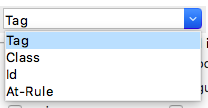
\includegraphics[scale=0.6]{typeselect}
\end{center}
A display selector is also available. It alows the user to see only the selected definition, or only the unselected definition. To access to this parameter go to center top menu.
\begin{center} 
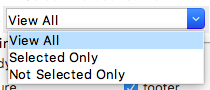
\includegraphics[scale=0.6]{viewselect}
\end{center}
In order to make fast modification on selection, another selector is also available. 
\begin{center} 
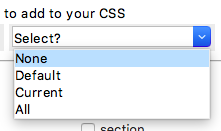
\includegraphics[scale=0.6]{selectionselect}
\end{center}
This one gives four selection preset:
\begin{itemize}
\item[None:]All the definitions in the current Type, View and Search selection will be unselected
\item[Default:] Set all the definitions in the current type selection to the default setting
\item[Current:] This state is automaticly set once the user start modifying the definition selection
\item[All:]All the definitions in the current Type, View and Search selection will be selected\\
\end{itemize}
Then, on the top right comes a search bar. The search bar will display every definition in the Type and View selection which contains the text typed.
\begin{center} 

Note:
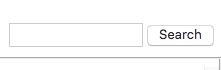
\includegraphics[scale=0.6]{searchbar}
\end{center}
\newpage
\section {StepWarning}
The Warning Step is meant to give information to the users to optimize the CSS file. Thanks to those warnings the users can edit the HTML\&CSS files to make the new CSS file even lighter.\\

\begin{center} 
\includegraphics[scale=0.35]{stepwarning}
\end{center}
\begin{itshape}
Note: The warning step doesn't block the generation process, it is possible to generate the CSS file with warning. Also, the program by itself, doesn't apply any modification based on those warnings.\\
\end{itshape}
\\This tab is divided in two parts:\\
\\On the top comes a hide bar, if the users want to hide warnings about a particular definition, they just have to add the exact name add press 'Enter' or click on refresh. If they want to remove all definitions containing a specific character patern, they have to type example*.\\
This command will remove all warnings concerning definition part named example\\
\\On the bottom, warnings are displayed. There are three types of Warning:\\
\begin{itemize}
\item The first one, warns the users that they are using in their HTML file, a Tag, Class or Id which is not defined in the CSS files given.
\item The second one, warns the users that a Tag, Class or Id is defined more than one time in the original CSS files. This may be normal or not. Microchip-CSS-Optimizer will not gather the definitions, and so, in order to make the new CSS file even lighter, the users may have to manually edit the generated CSS file to merge those definitions.
\item The third one, warns the users that a particular definition is not oftenly used in the HTML files, and so, removing it's definition may lighten the new CSS file.
\end{itemize}
\newpage
\section {Step3}
Step3 is the generation part. To generate an optimized CSS file, press Generate. If you want to make the CSS file even lighter press generate .min. This file will be lighter but almost unreadable. The Select file button allow the users to restart the process from scratch.
\begin{center} 
\includegraphics[scale=0.35]{step3}
\end{center}
\part {Known Issues}
\setcounter{section}{0}
Some issues may appear at the end of the optimization. The generated CSS file may not be working properly after conversion. The main reason is that this program is really conservative in its way to add definition by default. So here is a list of definition to manually add, that may fix display issues after conversion.
\section {Bootstrap}
\begin{itemize}
\item [Bootstrap 3 \& 4:] If you encounter a graphic issue where elements are added horizontaly instead of verticaly after conversion, this may be caused by a missing definition called .row[after]. This definition is stored in the Class tab. Use Search bar to get a fast acess to it.
\end{itemize}
\part {Extra}
\setcounter{section}{0}
\section {Create a Shortcut}
\subsection{Mac}
\begin{itemize}
\item Create a new file named "Microchip-CSS-Optimizer.command"
\item Type in the file: Microchip-CSS-Optimizer
\item Save and close
\item type in command prompt:
\end{itemize}
\begin{mdframed}[backgroundcolor=black, fontcolor=white]
chmod u+x /path/to/Microchip-CSS-Optimizer.command
\end{mdframed}
where /path/to/ is the path to your new file.

\subsection{Windows}
\begin{itemize}
\item Create a new file named "Microchip-CSS-Optimizer-Launcher.bat"
\item Type in the file:start Microchip-CSS-Optimizer
\item Save and close
\end{itemize}
\section {Add commands to windows command prompt}
Window command prompt works with environment variables. Those environment variables are stored in .exe files placed anywhere on the computer. Windows will store the paths of those .exe files in a file to get acess to them. Once you type a command, the command prompt will try each .exe file until it find yours. Pip on windows is a .exe file stored in the Script folder in Python installation diretory. To tell windows this .exe file has to be added to the environment variable, we need to edit the path file.
To do so, type in windows command prompt:
\begin{mdframed}[backgroundcolor=black, fontcolor=white]
setx PATH "\%PATH\%;C:\textbackslash Path\textbackslash To\textbackslash Python\textbackslash Install\textbackslash Scripts"
\end{mdframed}
Where:
\begin{itemize}
\item PATH is the file where the paths are stored
\item \%PATH\% represent all the old reference that we keep
\item ; a spacer between old and new path
\item C:\textbackslash Path\textbackslash To\textbackslash Python\textbackslash Install\textbackslash Scripts is the path of your script folder in the Python directory. You shall only edit this part of the commandline and put your path. If you didn't change anything in Python installation paths, this path should be: C:\textbackslash PythonXX\textbackslash Scripts
\end{itemize}
\begin{itshape}
Note: After this, you need to restart the command prompt, to apply changes.
\end{itshape}

\section {Move into file system with command prompt}
When you type a command in the command prompt, this command is always executed from a directory. That means that when you want to use commands dealing with files, the path to these files will have to be from the current directory to the file, and NOT the absolute path of these files.\\
If you want to know in which directory your command prompt is, type:
\begin{mdframed}[backgroundcolor=black, fontcolor=white]
pwd \hfill(For Mac and Linux)\\
echo \%cd\% \hfill(For Windows)
\end{mdframed}
If you want to change the current directory, use:
\begin{mdframed}[backgroundcolor=black, fontcolor=white]
cd .. \hfill(To go to the parent folder)\\
cd MyFolder \hfill(To go inside MyFolder)
\end{mdframed}
If you want to know what folders and files are in your curent directory just type:\\
\begin{mdframed}[backgroundcolor=black, fontcolor=white]
ls\hfill(For Mac \& Linux)\\
dir \hfill(For Windows)
\end{mdframed}
\end{document}